\documentclass{article}

\usepackage{simcmag}
\usepackage[export]{adjustbox}

\date{\hspace{30mm}}
\currentvolume{2}

\newcommand{\simcmagcredits}{
  \footnotesize
  \begin{tcolorbox}[boxrule=1.0pt,colback=white,hbox,before upper*=\begin{tabular}{l},after upper*=\end{tabular}, sharp corners,left=-5pt,right=-5pt]
  Editor-in-Chief: Edward Y. \\
  Editor: Cecilia S. \\
  Staff Writers:\\
  \begin{tabular}{ll}
    Cecilia S. & Edward Y. \\
    Joyce H. & Michael Y.\\
    Owen X. & Rohan D. \\
    William Y. F. & William G. 
  \end{tabular}
  \end{tcolorbox}
}

% uasage of picinpar:
%\begin{window}[1,l,\includegraphics{},caption]xxxxx\end{window}

% usage of window:
% \begin{window}[2,r,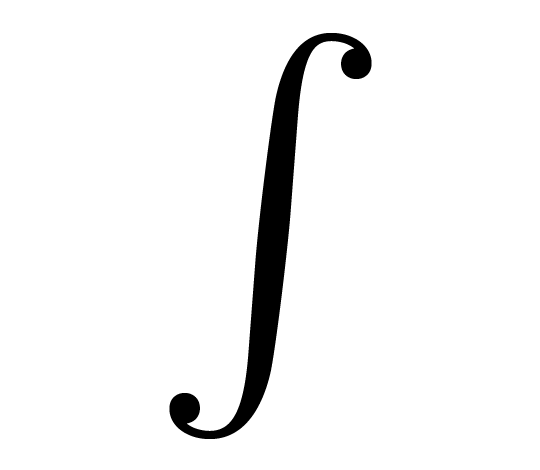
\includegraphics[width=1.0in]{img/logo.png},\centerline{a picture}]
% Duis aute irure dolor in reprehenderit in voluptate velit esse cillum dolore eu fugiat nulla pariatur. Excepteur sint occaecat cupidatat non proident, sunt in culpa qui officia deserunt mollit anim id est laborum
% \end{window}

%%%%%%%%%  Front matter   %%%%%%%%%
\begin{document}
\maketitle
\begin{minipage}[t]{.45\textwidth}\thispagestyle{empty}
  \vspace{-11mm}
  \tableofcontents
\end{minipage}% 
\begin{minipage}[t]{.1\textwidth}\thispagestyle{empty}
  \;
\end{minipage}% 
\begin{minipage}[t]{.45\textwidth}\thispagestyle{empty}
  \footnotesize
  \setlength{\parskip}{5pt}
  \vspace{-7mm}
  {\itshape
  Congratulations to the following students for being the top scorers at Seattle Infinity Math Competition 10!
    \begin{center}
        \begin{tabular}{c c c}
        \hline
           \textbf{In-Person}   & \textbf{Name} & \textbf{Score} \\
           1 & Eric Yee & 132  \\
           2 & Benjamin Fu & 126 \\
           3 & Vishnu Mangipudi & 123 \\
           4 & Jason Yao & 109.5 \\
           5 & Leya Balayoghan & 106.5 \\
           6 & Eason Xu & 103.5 \\
           \hline
        \end{tabular}
    \end{center}
    
    \begin{center}
        \begin{tabular}{c c c}
        \hline
          \textbf{Online}    & \textbf{Name} & \textbf{Score} \\
           1 & Jiahe Liu & 145.5  \\
           2 & [Anonymous] & 132 \\
           3 & Faizaan Siddique & 127.5 \\
           4 & Catherine Xu & 121.5 \\
           5 & William Liu & 115.5 \\
           5 & [Anonymous] & 115.5 \\
           \hline
        \end{tabular}
    \end{center}
}
\end{minipage}

\vspace{3mm}


\begin{multicols}{3}

\articletitle{A Lanyard Puzzle}{Cecilia Sun}{}
%\begin{center}
%    \includegraphics[scale=0.6]{img/Vol2/lanyard11.png}
%\end{center}
%removing for spacing reasons

Recently, I spent 5 weeks at Canada/USA Mathcamp. Being surrounded by math kids, our mealtime chatter frequently included spirited conversations about some interesting math puzzle or problem. Out of all the problems we pondered, one of the puzzles that caused the most lively dinnertime discussions was what we called the lanyard puzzle. It’s most commonly known as the Picture-Hanging puzzle, but, being at camp and having an abundance of lanyards (we each had one to hang the various keys and cards given to us by the university), we called it the lanyard puzzle. 

The most simple formation of the puzzle is as follows: suppose you have two pegs, and you want to hang the lanyard around these pegs such that removing either peg causes the lanyard to fall. Is this possible? If so, how? 

If you spend some time experimenting, you might come up with the following configuration, which is indeed a solution to the puzzle:

\begin{center}
    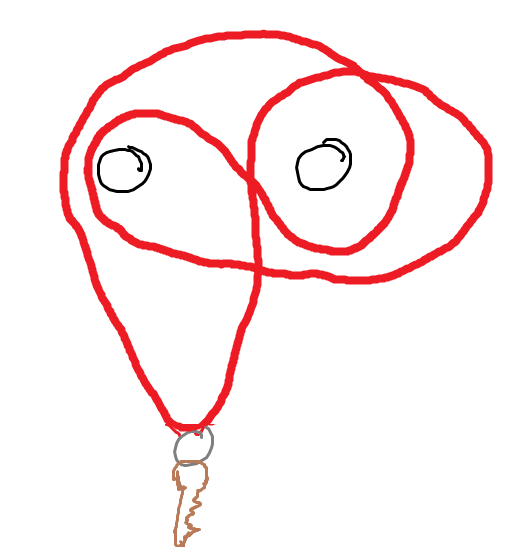
\includegraphics[scale=0.4]{Magazines/img/Vol2/lanyard2.png}
\end{center}

After finding this solution, you might be inclined to see if we can generalize this to more pegs: for instance, can we hang a lanyard from three pegs such that removing any singular peg causes the lanyard to fall? What about four pegs? $n$ pegs? As it turns out, the answer is yes, but to see this we first return to the two-peg case to see what is really going on. 

Firstly, let's name our pegs $A$ and $B$. 

\begin{center}
    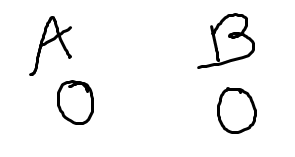
\includegraphics[scale = 0.6]{Magazines/img/Vol2/lanyard3.png}
\end{center}

Observe that, while hanging the lanyard, we only really have four distinct moves: wrapping the lanyard around peg $A$ clockwise, wrapping it around peg $A$ counterclockwise, wrapping it around peg $B$ clockwise, and wrapping it around peg $B$ counterclockwise. Let’s call these operations $A$, $A’$, $B$, and $B’$ respectively. Thus, we can express each hanging configuration as a string of these four operations. 

\begin{center}
    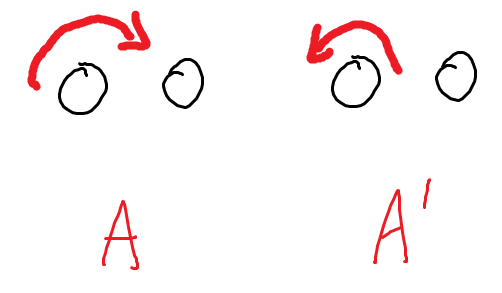
\includegraphics[scale=0.4]{Magazines/img/Vol2/lanyard41.png}
    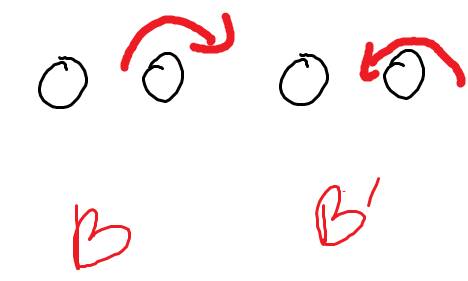
\includegraphics[scale=0.4]{Magazines/img/Vol2/lanyard42.png}
\end{center}

From here we make two observations:

Firstly, if we ever have $A$ and $A’$ right next to each other, they cancel each other out. The same applies to $B$ and $B’$.

%\begin{center}
%    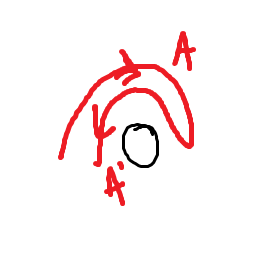
\includegraphics[scale=0.6]{Magazines/img/Vol2/lanyard5.png}
%\end{center}

Secondly, removing a peg removes all operations associated with that peg from the string. So, removing peg $A$ will cause all instances of operation $A$ or $A’$ to be removed from the string. 

If we look at our solution, we can write out the sequence of operations it’s associated with: 

\begin{center}
    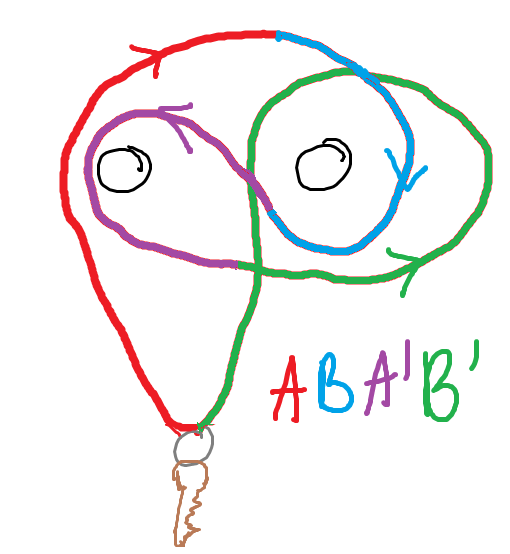
\includegraphics[scale=0.4]{Magazines/img/Vol2/lanyard6.png}
\end{center}

Note that removing all the $B$’s will reduce the sequence to $AA’$ which cancels into nothing, meaning the lanyard drops; the same is true for removing the $A$’s.

From here, we have a sufficient framework to examine cases in which there are more pegs.

Firstly, for notational ease, let's rename the pegs to pegs $1$, $2$, $3$, $\dots$. We denote hanging the lanyard clockwise around peg $n$ to be $x_n$, and hanging the lanyard counterclockwise around peg $n$ to be $x_n^{-1}$ (under this notation, it is also clearer that looping clockwise and counterclockwise around the same peg are ``inverse" operations). Let's also let $S_n$ denote the sequence of operations around the first $n$ pegs that causes the lanyard to drop upon removing any of the first $n$ pegs. So, $S_2=x_1x_2x_1^{-1}x_2^{-1}$ and we want to find $S_3$.

Our work for the $2$-peg case is actually useful here! If, for example, we put $S_2$ ``between" $x_3$ and its inverse, $x_3^{-1}$, then removing either $A$ or $B$ will cause $S_2$ to cancel out, after which the $x_3$ and $x_3^{-1}$ will be next to each other and cancel each other out.

But we run into an issue when peg 3 is removed -- the string becomes $S_2$, which does not fall off the peg! If we find a configuration (which we will call $S_2^{-1}$) to put after the $x_3^{-1}$ such that $S_2S_2^{-1}$ cancels out, then we win! 
It turns out that we can just directly do this; we start at the last operation in $S_2$ and take its inverse, then continue appending the inverse of the operation from right to left until we reach the end.

For example, to invert $x_1x_2x_1^{-1}x_2^{-1}$, we start at the right end, with the inverse of $x_2^{-1}$ (which is just $x_2$). Then we go to the next operation (moving left) with the inverse of $x_1^{-1}$ (so, our string is now $x_2x_1$); eventually, we end up with $S_2^{-1}=x_2x_1x_2^{-1}x_1^{-1}$. 

We can also check that $S_2S_2^{-1}$ completely cancels out:

\begin{align*}
	S_2S_2^{-1}&= x_1x_2x_1^{-1}x_2^{-1}x_2x_1x_2^{-1}x_1^{-1} \\
	&= x_1x_2x_1^{-1}(x_2^{-1}x_2)x_1x_2^{-1}x_1^{-1} \\
	&= x_1x_2x_1^{-1}x_1x_2^{-1}x_1^{-1} \\
	&= x_1x_2(x_1^{-1}x_1)x_2^{-1}x_1^{-1} \\
	&= x_1x_2x_2^{-1}x_1^{-1} \\
	&= x_1(x_2x_2^{-1})x_1^{-1} \\
	&= x_1x_1^{-1}
\end{align*}

Now that we have verified that $S_2^{-1}$ does indeed exist, we arrive at the final construction $S_3=S_2x_3S_2^{-1}x_3^{-1}=x_1x_2x_1^{-1}x_2^{-1}x_3x_2x_1x_2^{-1}x_1^{-1}x_3^{-1}$.

\begin{center}
    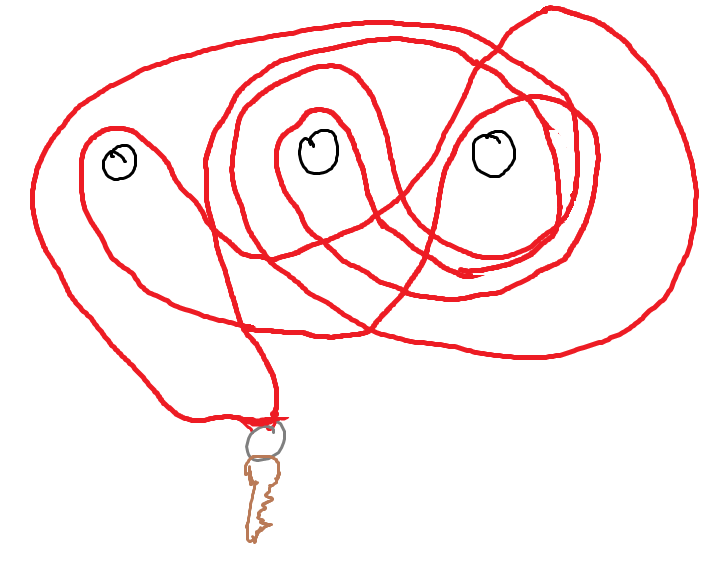
\includegraphics[scale = 0.4]{Magazines/img/Vol2/lanyard71.png}
\end{center}

We can, in fact, generalize this to any number of pegs; for $S_4$ we can take $S_3x_4S_3^{-1}x_4^{-1}$ to get the extremely lengthy construction
$S_4=x_1x_2x_1^{-1}x_2^{-1}x_3x_2x_1x_2^{-1}x_1^{-1}x_3^{-1}x_4x_3x_1$ $x_2x_1^{-1}x_2^{-1}x_3^{-1}x_2x_1x_2^{-1}x_1^{-1}x_4^{-1}$. To get $S_n$ we can take $S_{n-1}x_nS_{n-1}^{-1}x_n^{-1}$. This is what we call a \textit{recursive construction}, since our construction for $n$ pegs depends on the construction for $n-1$ pegs. 
So, it turns out for \textbf{any number of pegs} there always exists a way to wrap a lanyard around all the pegs such that the picture hangs when all the pegs are intact, but drops once any single peg is removed---we just might need a really long string!

At this point, my friends and I had solved the puzzle (and finished our dinners), but we weren’t quite satisfied yet, due to a small issue -- we could easily demonstrate the 2-peg configuration by wrapping our lanyards around our fingers; the 3-peg configuration was trickier because it had more operations and thus required a lot more wrapping, but once we got to 4 pegs the lanyard was simply too short and the number of operations (22) too large to demonstrate it physically.

Our construction is indeed pretty inefficient in terms of the number of operations in each $S_n$; in fact, each time we add a new peg, we more than double the number of operations (since we include a copy of both $S_{n-1}$ \textbf{and} $S_{n-1}^{-1}$); the number of operations is growing exponentially under this construction!

However, it turns out that there is a more efficient way to recursively build up $S_n$. The key idea is to keep the format 

The idea is to keep the $ABA^{-1}B^{-1}$ format, but instead try to have $A$ and $B$ be more balanced. Instead of having one of $A$ and $B$ account for just one peg and the other account for all the rest of the pegs, we split the pegs into two groups as evenly as we can and have $A$ account for the first group of pegs (in other words, $A$ will be the sequence for which removing any single peg within the first group of pegs will completely cancel $A$ out) and $B$ account for the second group of pegs. This way, instead of constructing $S_n$ in terms of $S_1$ and $S_{n-1}$ we instead construct it in terms of $S_{\lfloor n/2\rfloor}$ and $S_{\lceil n/2 \rceil}$. 

\begin{center}
    
\includegraphics[scale = 0.8]{Magazines/img/Vol2/lanyard1.png}
\end{center}

\closearticle
\clearcolumn

\articletitle{Special Numbers in Euler’s Identity}{Joyce Huang}{}

In math, not all numbers are of equal importance. Some have very special and unique properties that constantly show up in formulas and theorems. Five of these special numbers are $0$, $1$, $i$, $\pi$, and $e$.

\begin{center}
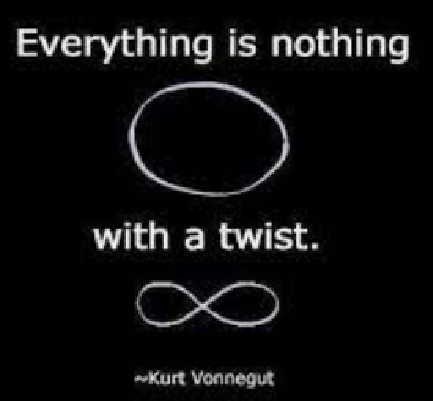
\includegraphics[scale=0.6]{Magazines/img/Vol2/specialnum0.png}
\end{center}

$0$ represents the quantity of nothing. Societies from all over the world invented the concept independently millennia ago, and it is extremely unlike any other number. 0 is neither positive nor negative, it cannot be a divisor, and so much more. It is also an additive identity, meaning   $x + 0 = x$ for all $x$. 


$1$ represents a single unit or quantity. The first natural number, it too is very special. $1$ is neither prime nor composite and it only has one divisor, which is itself. Also, $1$ is a multiplicative identity, meaning $x\times 1 = x$ for all $x$. 

For a long time, it was accepted as fact that the square of every number is nonnegative, and that one cannot take the square root of a negative number. However, the introduction of the number $i$ into mathematics brought about entirely new branches of math and countless new discoveries. $i$ is the square root of $-1$, and is called an imaginary number. Numbers of the form $a + bi$, where a and b are real numbers, are called complex numbers, and can be graphed on a coordinate plane. So, the discovery of $i$ quite literally introduced a whole new dimension of numbers.
\begin{center}
    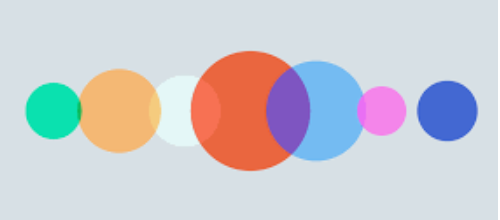
\includegraphics[scale=0.8]{Magazines/img/Vol2/specialnum2.png}
\end{center}
As mathematicians began to study circles, their curiosities were sparked by the relationship between different lengths in a circle, namely the ratio between the circumference and the diameter. It seemed that no matter the size of the circle, the ratio was always the same, so the question shifted to finding the exact value of that ratio. Of course, the exact value could never have been found, since $\pi$ is an irrational number. It is also a transcendental number, meaning it is not the root of any polynomial of finite degree with rational coefficients. $\pi$ has become one of the most well-known irrational numbers, with most people knowing at least several of its first digits and others striving to memorize as much of it as they can for fun.
\begin{center}
    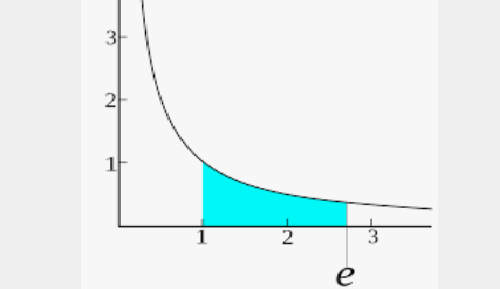
\includegraphics[scale=0.8]{Magazines/img/Vol2/specialnum3.png}
\end{center}
The constant $e$, also known as Euler’s number, has been widely used in number theory, algebra, statistics, and more since the early 17th century. Swiss mathematician Jacob Bernoulli discovered its value in 1683, but it had been referred to in a list of logarithms in base $e$, the natural logarithm, as early as 1618.

When Bernoulli discovered e, he had been trying to find the value of
\[\lim_{n\rightarrow\infty} \left(1+\frac{1}{n}\right)^n.\]
This expression might look familiar to you; Bernoulli discovered it while studying compound interest. As the frequency the interest is added to a starting value of $\$1$ increases infinitely, the money approaches $\$2.71828…$, which is the value of $e$. 

Another Swiss mathematician, Leonhard Euler, became engrossed in the number and discovered that it is the value of the sum.
\[e=\sum_{n=0}^{\infty}\frac{1}{n!}=1+\frac{1}{1}+\frac{1}{1\cdot 2} + ...\]
Euler also had many more discoveries related to $e$, including Euler’s formula, 
\[e^{ix}=\cos x + i\sin x,\]
a special case of which is \emph{Euler’s identity}.

\begin{center}
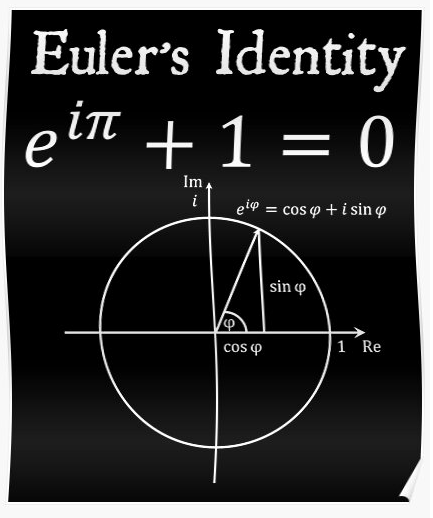
\includegraphics[scale=0.75]{Magazines/img/Vol2/specialnum1.png}
\end{center}

Euler’s identity is Euler’s formula when $x = \pi$. The equation then becomes
\[e^{i\pi}+1=0.\]

One might notice that there are 5 distinct numbers in this equation, and they happen to be the special numbers discussed in the article! Not only that, this identity includes each of the basic arithmetic functions addition, multiplication, and exponentiation exactly once. 

Euler’s identity is truly very special and combines five very special elements in it.

\closearticle

\articletitle{Imaginarily Complex; Really Simple}{Rohan Dhillon}{}
You’ve probably heard of complex numbers before—good old formulas like $i=\sqrt{-1}$, $z=a+bi$, and $|z|=a^2+b^2$ hopefully ring a bell (if they don’t, this article might be pretty confusing). But did you know that complex numbers have a lot of use beyond just the confusion of high school students? In fact they’re used in everything from counting sums to describing our universe. 

But we’re getting ahead of ourselves. First we really need to understand complex numbers at the fundamental level—and I mean very fundamental. Why did we come up with them anyway? In the 1500s, we still didn’t know how to solve a cubic equation in full. The primary problem was that square roots of negative numbers kept popping up everywhere—at the time, no one had conceived of an imaginary number. However, an Italian mathematician by the name of Gerolamo Cardano decided to let $\sqrt{-1}$ exist as a concept. When he did, the solutions to a depressed cubic, a special type of cubic whose $x^2$ coefficient is $0$, fell into place immediately. 
\begin{center}
    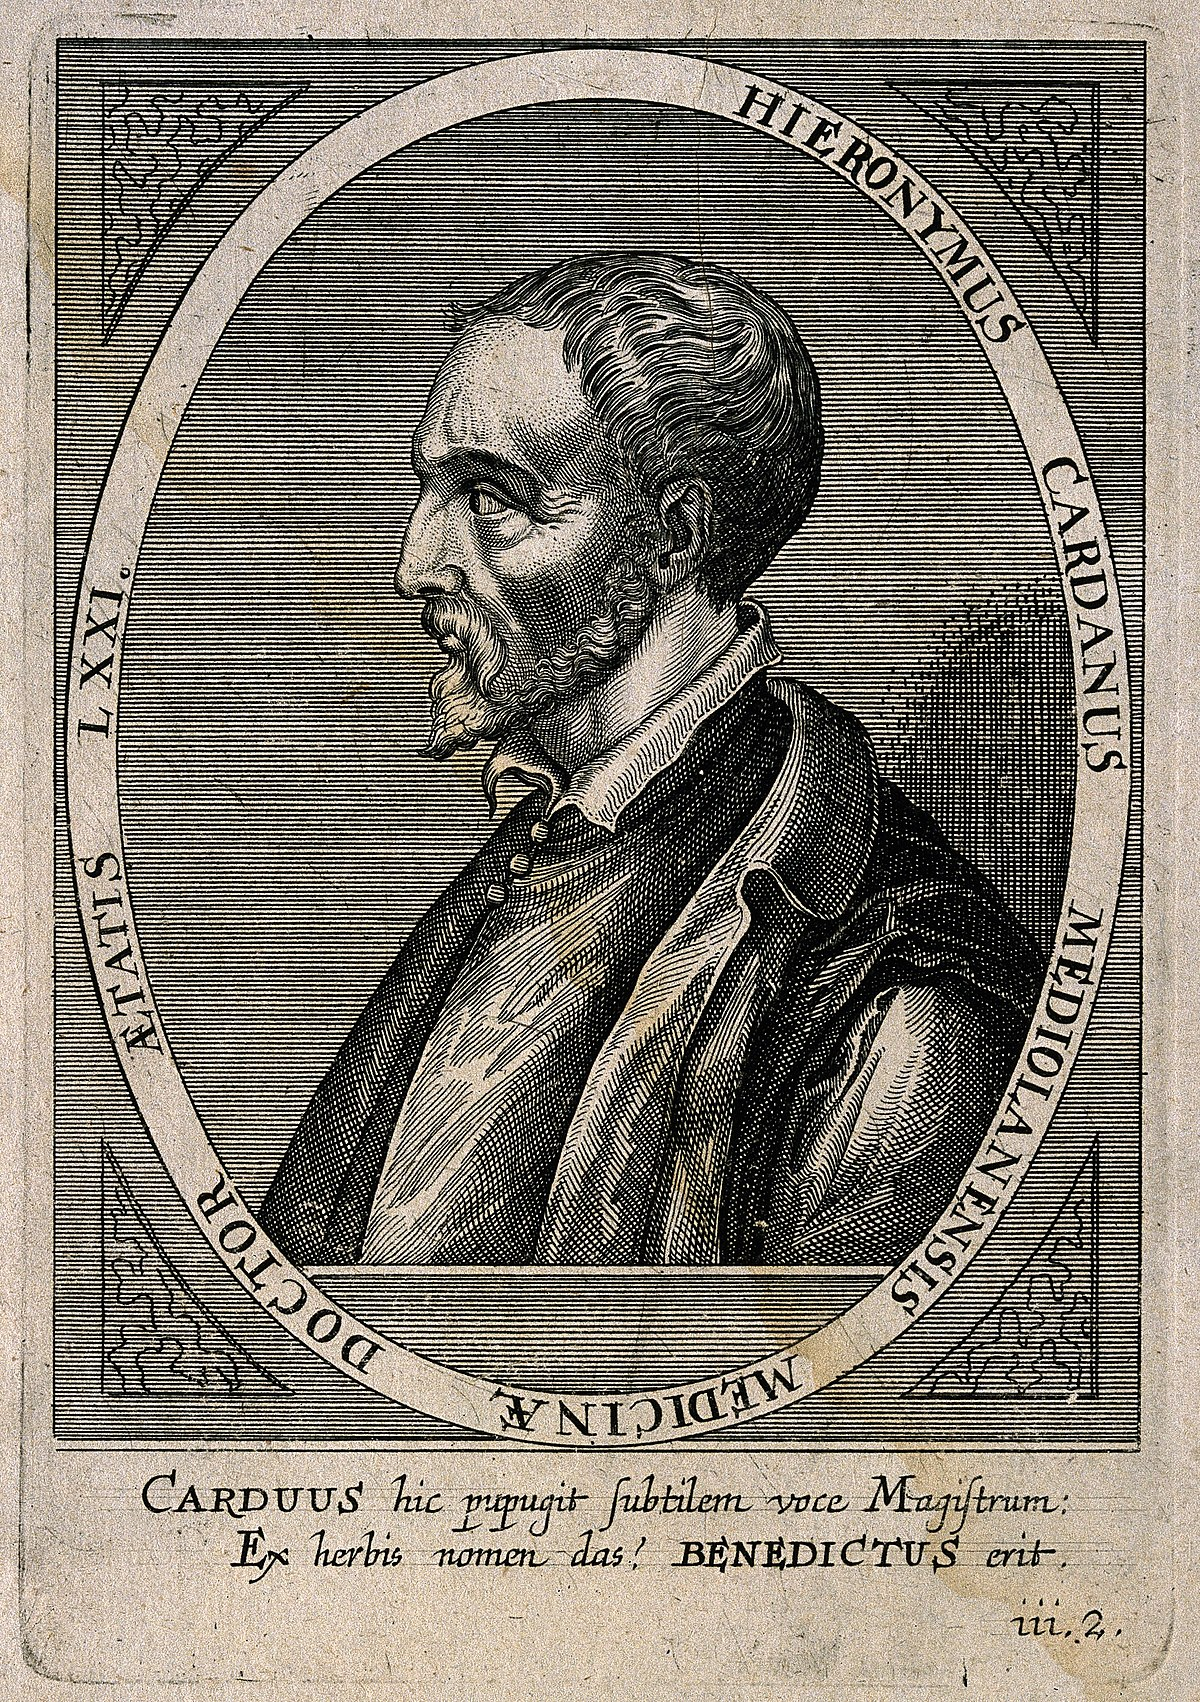
\includegraphics[scale=0.1]{Magazines/img/Vol2/gerolamo.jpg}
\end{center}
And then, some centuries later on, we came up with the Fundamental Theorem of Algebra which states that any polynomial equation of degree $n$ has $n$ roots (some can be repeated). But then what are the roots of, say, $x^7=1$? Here’s where we have to think of complex numbers differently. Rather than defining $z=a+bi$, let’s define it as $z=(r,\theta)$, where $r=|z|$ and $\theta$  is the angle the complex number makes with the positive $x$-axis counterclockwise. (This definition is akin to treating a complex number as a point in polar coordinates). 

With this idea in mind, we have a very useful formula for the multiplication of complex numbers (which we won’t prove): DeMoivre’s Formula: $pq=(r_pr_q,\theta_p+\theta_q)$. Basically, we multiply magnitudes and add angles. So if we take powers we should get $z^n=(r^n,n\theta)$. 
\begin{center}
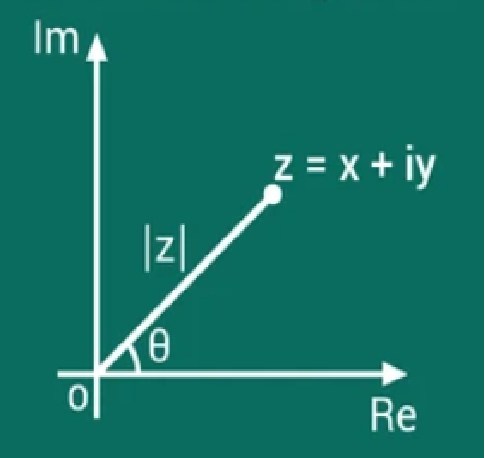
\includegraphics[scale=0.8]{Magazines/img/Vol2/complex1.png}
\end{center}
One is also a complex number, however, with $1=(1,0)=(1,2\pi)=(1,4\pi)$.... So we’re looking for all complex numbers x such that $x^7=(r^7,7\theta)=(1,2\pi k)$. Well, since $r$ is always a positive number, $r=1$ and for , we can just divide by $7$ to get $\theta=\frac{2\pi k}{7}$. Thus, we have our seven solutions as promised. These seven solutions are called the seventh roots of unity. In general, all of the solutions to $x^n=1$ are called $n$th roots of unity. 

So complex numbers are made to solve algebraic (usually polynomial) equations. But in how many ways can we really use this fact? It’s not like some counting problem could be solved with complex numbers right? Well…that’s the funny thing. There’s a few important problems that can. One of the more famous one (at least in math competition circles) is one variant of the following:

\textit{Suppose we choose a subset of numbers from {1,2,...,100}. What is the probability they sum to a multiple of 5?} The first thing we need to do is create a \textit{generating function}. These essentially turn finding the numbers of ways to count something into finding the coefficients of a polynomial. For our problem, the generating function is 
$$g(x)=(x+1)(x^2+1)...(x^{100}+1).$$ 
Each term $x^n+1$ says that we can either choose $n$ or $1$. When we multiply everything out, the coefficient of each term tells us the number of ways to get it. For example, the constant term is $1=1x^0$ meaning there is one way to get a sum of $0$. Meanwhile, the $x^{5050}$ coefficient is also $1$, meaning there’s one way to get a sum of $5050$. 

Okay, so all we need to do is find the sum of the coefficients of $x^5,x^{10},x^{15},...,x^{5050}$. Hmmmm…that doesn’t seem easy…unless we use roots of unity. Let the five roots of unity to $x^5=1$ be $z_0=1, z_1=(1,72), z_2=(1,144), z_3=(1,216), z_4=(1,288)$. Then, note that all of these roots of unity sum to $0$…and their squares sum to $0$…and their cubes sum to $0$…and their fourth powers too! But thankfully, since their fifth powers must all be $1$, their fifth powers sum to $5$. Aha! If we take $g(z_0)+g(z_2)+...+g(z_4)$, we get a nonzero sum only on fifth powers. This is exactly what we want! So all we need to do is find the above sum and divide it by $5$! But…how do we do that? 
	
Let’s take one root of unity—say $z_1$ for simplicity (note that taking $1$ will just give us $2^100$). Then, we want $(z_1+1)(z_1^2+1)(z_1^{100}+1)=[(z_1+1)(z_1^5+1)]^20$ since after taking the root to the sixth power, we arrive back at the original root. All we need to do is find the thing inside of the square brackets. Now, we turn away from polar notation and back into our $a+bi$ form. Doing this gives us $z_1=\cos 72+i\sin 72, z_2=\cos 144+i\sin 144$, and so on. 
\begin{center}
    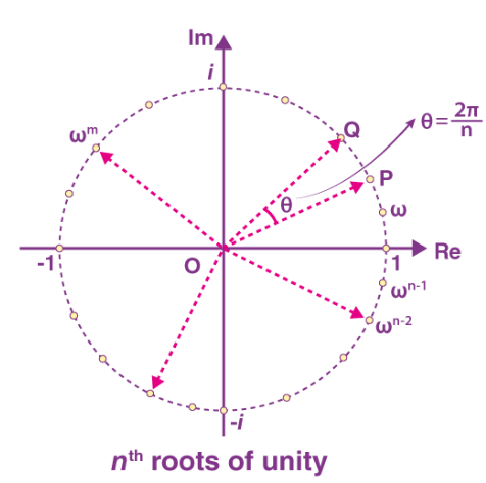
\includegraphics[scale=0.7]{Magazines/img/Vol2/root1.png}
\end{center}
But now notice that $z_4=\overline{z_1}, z_3=\overline{z_2}$, and adding the real number $1$ to those quantities won't change anything. Thus what we really want is 
$z_1\overline{z_1}z_2\overline{z_2}\cdot 2=|z_1|^2|z_2|^2\cdot 2$. 

This is just 
\begin{align*}
 & [(1+\cos 72)^2+\sin^2 72)  \cdot   \\
 & ((1+\cos 144)^2+\sin^2 144]  = \\
 & [2+2\cos 72][2+2\cos 144]  = \\
 & 4(1+\cos 72+\cos 144+\cos 72 \cos 144)
\end{align*}


From here the only way to really proceed is to know that $\cos 144=-\cos 36$, $\cos 18=\frac{1+\sqrt5}{2}$, and $\cos 2\theta=2\cos^2 \theta -1$. Plugging all of these things in and slogging through the arithmetic we get that our expression is $2$—exactly. Then, our $20$th power expression is $2^20$, and our answer is simply $\frac{4\cdot 2^{20}+2^{100}}{5}$ ways — a little more than exactly a fifth. 
And there you have it—imaginary numbers solving a very \emph{real} problem (okay, maybe not that real but you get the point). I hope that you’ve gotten a sense of just how powerful this topic is—and that was just the introduction. Complex numbers have a special place in geometry problems, where they simplify arithmetic, and in quantum mechanics, where they quite literally define how particles behave. So there you have it: complex numbers—conceived in a mathematician's head, but known by the universe for 13.8 billion years. 
\begin{center}
    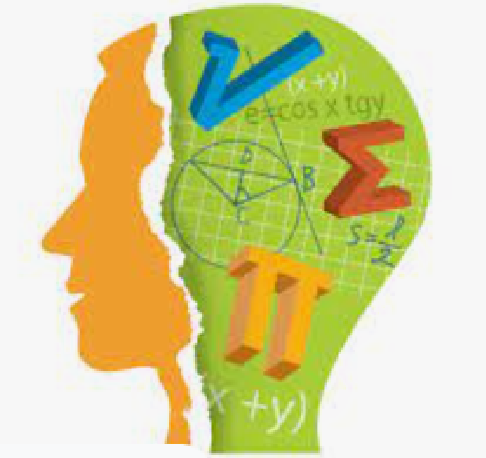
\includegraphics[scale=0.7]{Magazines/img/Vol2/root2.png}
\end{center}
\closearticle

\articletitle{An Introduction to Elliptic Curves}{William Gvozdjak}{}
Elliptic curves are one of the excitements of the research math world right now. For example, Fermat’s Last Theorem, a notorious and extremely difficult result in number theory, was finally proven after over three centuries using elliptic curves. What really are elliptic curves, and why are they useful?
\begin{center}
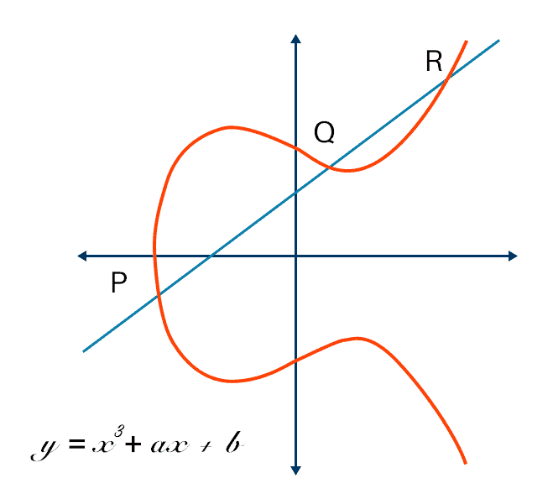
\includegraphics[scale=0.8]{Magazines/img/Vol2/curve3.png}
\end{center}
We first present an introductory question: is there a quick way to generate all primitive Pythagorean triples? In other words, is there an efficient method to generate all triples of positive integers $(a, b, c)$ where $c^2=a^2+b^2$, and $\gcd(a, b, c)=1$? How many solutions are there?

To answer this question, note that we can divide the above equation by $c^2$, giving us $1=\left(\frac{a}{c}\right)^2+\left(\frac{b}{c}\right)^2$. This is significant because this equation is now in the form of the equation of the unit circle! Therefore, we have shown that there is a one-to-one correspondence between primitive Pythagorean triples and ``rational points’’ with positive coordinates on the unit circle in the coordinate plane: points on the unit circle where both coordinates are positive, rational numbers.


How can we use this to general all primitive Pythagorean triples? We use a \textbf{projector}: we take an existing rational point, draw a line through that point, and use the second intersection of that line and the circle (``project’’ that point to another point on the circle). Our initial point will be a simple solution, such as $(-1, 0)$:

\begin{center}
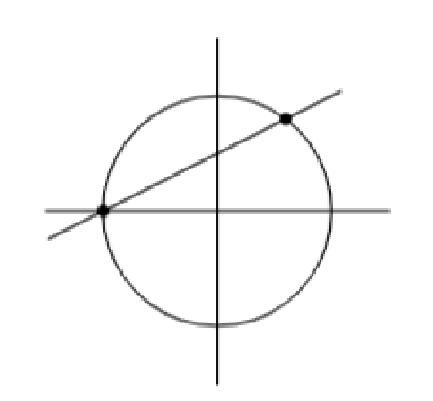
\includegraphics[scale=1]{Magazines/img/Vol2/curve1.png}
\end{center}

This new point must also be a rational point! This is not hard to show – we can solve the equation of the circle with the line, giving us a quadratic equation with rational coefficients. By Vieta’s formulas, as one solution is rational, the other solution must also be rational. Also, note that simply by varying the slope of the line that we project through to all rational numbers, we can actually generate \textit{all} rational solutions to $1=x^2+y^2$: if there is a rational point on $x^2+y^2=1$, then we can simply take the line through it and the point $(-1, 0)$ (this line is guaranteed to have rational slope).

Therefore, we have found a systematic way to find all primitive Pythagorean triples: take all lines with rational slope through the point $(-1, 0)$ and intersect them with the circle $x^2+y^2=1$, with the solutions with positive $x$ and $y$ coordinates resulting in primitive Pythagorean triples. Notice that this also proves that there are an infinite number of primitive Pythagorean triples, as there are an infinite number of rational numbers that we can choose as the slope.

Now, we look at a more complex problem. What is the set of all primitive triangles that have integer side lengths, integer area, and two sides with lengths that are in the ratio $3$ to $4$? Using Heron’s formula and some transformations, it is possible to prove that all such solutions are classified by the equation
\[y^2=x(x-9)(x-16).\]


An equation of this form is known as an \textbf{elliptic curve}: an equation of the form $y^2=p(x)$, where $p(x)$ is a polynomial of degree $3$ with $3$ distinct roots. As we wish to again generate all rational solutions to this equation, we will turn to the strategy that we used earlier for the primitive Pythagorean triples: the ``projections,’’ by looking for some sort of operation that will allow us to generate another solution.

\begin{center}
    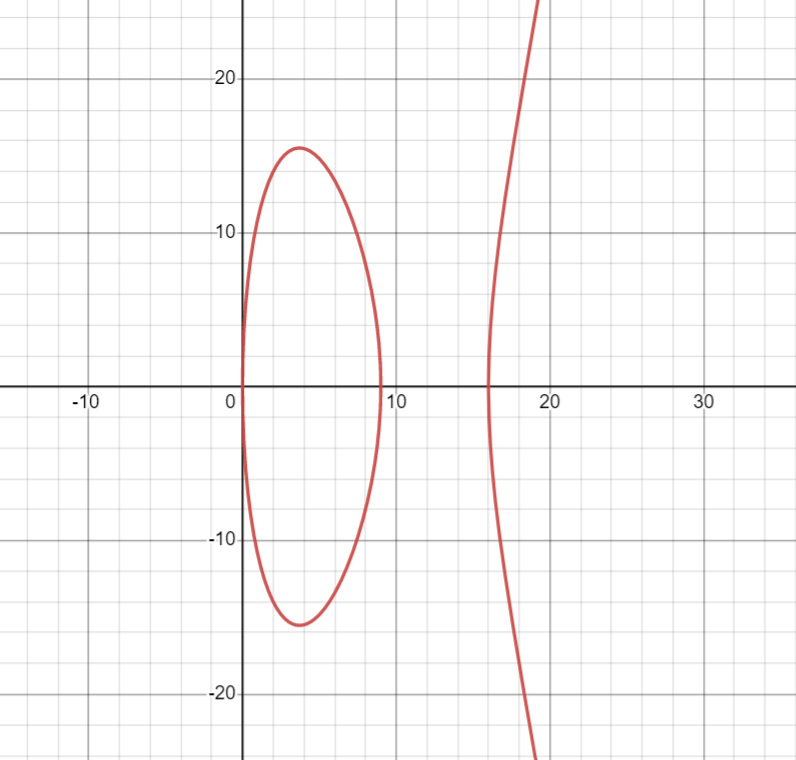
\includegraphics[scale=0.4]{Magazines/img/Vol2/ellipticCurves.png}
\end{center}

Inspired by our strategy with primitive Pythagorean triples, we may try to take a line and intersect it with the elliptic curve. Notice that if we do this, we end up with a cubic equation. However, unlike with the quadratic, this line not only needs to go through \textit{one} rational point, but \textit{two}: even if there is one rational solution, Vieta’s formulas does not guarantee that the last two solutions are necessarily rational. Therefore, we will define a new operation $\star$, which takes in two points $P$ and $Q$, and returns the third intersection point between the line $PQ$ and the elliptic curve. This requires some ``hacking’’ to rigorously define (e.g. what if $P=Q$, or $P$ and $Q$ have the same $x$-coordinate? Answering this requires the introduction of new ideas like a ``point at infinity’’), but this seems to satisfy most properties that we need.

\begin{center}
    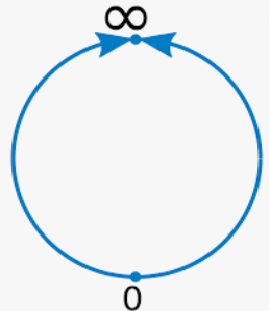
\includegraphics[scale=1.0]{Magazines/img/Vol2/curve4.png}
\end{center}

In reality, this operation behaves even nicer if we instead use the second intersection between the elliptic curve and the vertical line through $P\star Q$ (e.g. it behaves nicer with the point at infinity). Therefore, we have defined \textbf{elliptic curve addition}: the intersection of the elliptic curve with the vertical line through $P\star Q$. We have once again found a simple way to continuously generate solutions to our geometric problem with triangles!

This raises new questions: how long does the process of elliptic curve addition continue, until we start cycling back to points that we found before? Will it ever finish? Such ideas concern the \textbf{order} of elliptic curves. I highly encourage you to continue looking into such ideas and keep asking questions, as it appears that elliptic curves are the next big mathematical idea.
\closearticle

\articletitle{The Prime Number 57}{Edward Yu}{The Legend of the Grothendieck Prime}
\begin{center}
    \includegraphics[scale=0.4]{Magazines/img/Vol2/prime1.jpg}
\end{center}

It was another afternoon, and another lecture at math camp. The lecturer was explaining modular arithmetic in the context of finite fields—“say we have a prime number, like 57.” The audience chuckled, and someone said, “ooh, the Grothendieck prime!”

Alexander Grothendieck was one of the most prominent mathematicians of the twentieth century. Born in 1928, he grew up in the city of Berlin with anarchist parents who later fled the country in the wake of Nazism—leaving him in the care of a pastor in Hamburg. He ended up a refugee in France during World War II, and there he first became enamored with mathematics.

After the war ended, Grothendieck formally enrolled in college. There, he failed some of his classes (astronomy was one), but excelled in math. At one point, his mentor Lauren Schwartz—who had just won a Fields medal—gave him a list of 14 open questions at the end of his latest paper. In a few months, Grothendieck solved every single one, inventing novel mathematical methods in the process.

So what’s going on with 57, the so-called Grothendieck prime? There’s a legend about Grothendieck’s mode of mathematical thinking—its innovativeness lay in its abstraction, and it relied very little on examples. Once during a lecture, a student asked Grothendieck to work out a concrete example on a board with a particular prime number. “You mean an actual number?” Grothendieck asked. The student replied, “yes, an actual prime number,” to which Grothendieck said, “all right, take 57.” From then on, 57 (which, in case you haven’t noticed yet, is divisible by 3), became known as the Grothendieck prime.


Grothendieck was a theory-builder, not a problem-solver. He was add adjective known for an analogy about cracking a nut. The nut can be opened in one of two ways: either by smacking it with blunt force, or by soaking it in oil until the nut eases itself out of its shell. The first option felt unnatural, and almost barbaric to him; instead, he preferred using oil and water. In the words of mathematician and writer Jordan Ellenberg, “We have a word for difficult, and a word for easy, but we need a word for something about which it is difficult to understand that it is easy.” Grothendieck’s power was discerning easy problems cloaked in the mask of difficulty; he earned the Fields Medal in 1966.

Yet, in 1988, his golden period came to a sharp end. Grothendieck abruptly left his prestigious job, his practice of mathematics, and even his family. He withdrew to a remote French village to pursue a spiritual life as a recluse. In 2014, he died at the age of 86, but his groundbreaking work in algebraic geometry and K-theory lives on, most notably in Andrew Wiles’ proof of Fermat’s Last Theorem.

\begin{center}
    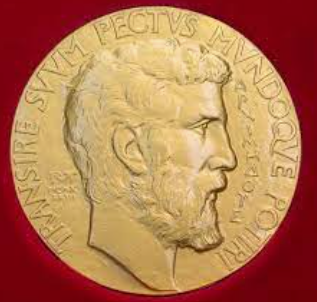
\includegraphics[scale=1]{Magazines/img/Vol2/prime2.png}
\end{center}

The next time you mistake 57 for a prime number, remember the man, the legend: remember Alexander Grothendieck.
\closearticle

\articletitle{Algorithmic number theory}{William Y. Feng}{Factoring Primes}
The security of the modern web depends, at a high level, on the so-called "irreversibility" of certain number-theoretic operations. These are operations are easy for computers do do one way but difficult to do in the opposite direction, and one such example is \textit{multiplication}---computers can multiply together two big numbers relatively quickly, but it takes much longer for them to find the factors of a given number. (This specific irreversible operation is key to the RSA cryptosystem.)

\begin{center}
    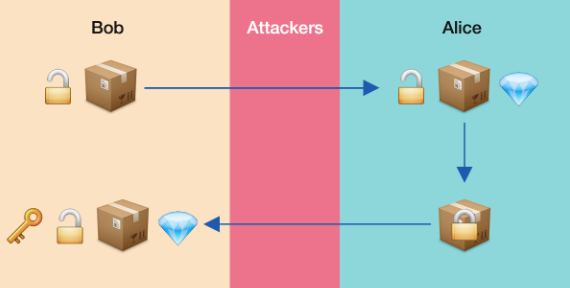
\includegraphics[scale=0.75]{Magazines/img/Vol2/algo1.png}
\end{center}

And while cryptography is one reason why we care about integer factorization algorithms, we might also care because they occasionally show up on math contests. As such, some of the methods discussed here are more practical for computers, while others are more practical for people.

\subsection*{Naive algorithm}

Suppose we are given a composite number $N$ that factors as $p \times q$. The most basic algorithm is brute force: try all the numbers from $2$ to $N - 1$, and see if they divide $N$. If $N = 2021$, we would go through $2, 3, 4, \dots, 42$ before finally discovering that $p = 43$ is a factor of $2021$. A helpful observation is that we can't have both $p > \sqrt{N}$ and $q > \sqrt{N}$, or $p \times q$ would be greater than $N$. Therefore, one of $p$ and $q$ is at most $\sqrt{N}$, so in this brute-force algorithm, we are guaranteed to hit a divisor of $N$ before $\sqrt{N}$.

\begin{center}
    \includegraphics[scale=0.2]{Magazines/img/Vol2/algo2.jpg}
\end{center}

If doing brute force manually, we can easily improve on this; instead of testing all the numbers from $2$ to $N - 1$, we can just test the \textit{primes}, because if a prime $p$ doesn't divide $N$, then none of its multiples can divide $N$ either. (Efficiently getting a list of primes is a nontrivial task for a computer and can be done with certain sieves or primality testing, but those are topics for another time.) For instance, instead of having to test all 42 numbers $2, 3, 4, \dots, 42, 43$ for divisibility into 2021, we just have to test the following 14 primes:
$$2, 3, 5, 7, 11, 13, 17, 19, $$
$$ 23, 29, 31, 37, 41, 43.$$
However, we might get unlucky and find a factor relatively late on in the list and have to check nearly all the primes up to $\sqrt{N}$ (which, by the , \href{https://en.wikipedia.org/wiki/Prime_number_theorem}{prime number theorem} is roughly $\sqrt{N}/(\log n)$ numbers).

If we don't find a factor early on, there's another strategy we can try.


\subsection*{Difference of squares (Fermat's method)}


Again, suppose $N$ is a composite number that we want to factor. By the difference of squares identity,
$$a^2 - b^2 = (a + b)(a - b),$$
if we can find $n$ and $m$ such that $n^2 - m^2 = N$, then we get a factorization for $N$ in the form $(n - m) \times (n + m)$. This motivates the following algorithm, called Fermat's method after French mathematician Pierre de Fermat:
\begin{enumerate}
    \item Guess $n^2$ as the smallest perfect square greater than $N$.
    \item If $n^2 - N$ is a perfect square, then let this be $m^2$, and we've found a factorization for $N$.
    \item Otherwise, increment $n$ by 1 and try again.
\end{enumerate}
In the case of $N = 2021$, we would first guess that $n^2 = 2025$ (with $n = 45$) and immediately get $n^2 - N = 4 = 2^2$, giving us the factorization with $(n, m) = (45, 2)$:
$$2021 = (45 + 2)(45 - 2) = 47 \times 43.$$
As another example, take $N = 8051$.  We notice that $90^2 = 8100$ is a perfect square that's slightly larger than 8051, so we can take $n = 90$ and get
$$n^2 - N = 8100 - 8051 = 49 = 7^2.$$
This gives us the factorization
$$(90 + 7)(90 - 7) = 89 \times 83.$$
If we used brute force, we would have had to test all the primes up to 83.
\begin{center}
    
\includegraphics[scale=1]{Magazines/img/Vol2/algo3.png}
\end{center}

In practice, Fermat's method is similar to brute-forcing primes, but starting from $\sqrt{N}$ instead of from 2. However, this is simpler to implement on a computer because of the relative ease of finding square roots as compared to making a prime sieve. Furthermore, using Fermat's method in combination with brute-force trial division is often faster than using either alone, especially when $N$ has small factors or factors close to $\sqrt{N}$.

\subsection*{Specialized manual factorization methods}

Here's a problem that I came across recently from the \href{https://artofproblemsolving.com/downloads/printable_post_collections/4092}{2014 National Internet Math Olympiad}:

\begin{center}
Find the sum of the prime factors of $67208001$, given that $23$ is one.
\end{center}

Let's first try to factor this with our standard methods. Trial division yields 3 and 7 as small prime factors, and we are also given that 23 is a factor. We can divide out by all three to get:
$$67208001 = 3 \times 7 \times 23 \times 139147.$$

We can now try to factor $N = 139147$ using Fermat's method. We want the smallest perfect square greater than $N$. As a rough bound, $139147$ is between $300^2 = 90000$ and $400^2 = 160000$, and we can do a bit of guess-and-check to narrow down $\sqrt{N}$ to between $370$ and $380$. We can then do  \href{https://en.wikipedia.org/wiki/Binary_search_algorithm}{binary search} to get that $\sqrt{N}$ is between $373$ and $374$.

Thus, the smallest perfect square larger than $N$ is $374^2$, and $374^2 - N = 729 = 27^2$. This gives us the factorization
$$139147 = (374 - 27)(374 + 27) = 347 \times 401.$$
We can check that 347 and 401 are both prime, so the answer is
$$3 + 7 + 23 + 347 + 401 = 781.$$
But that wasn't very enlightening! We had to calculate a lot of long divisions and find the square root of 139147. Surely this problem has intended solution that is less tedious.

\begin{center}
    
\includegraphics[scale=0.8]{Magazines/img/Vol2/algo4.png}
\end{center}


The idea is that we can rewrite $67208001$ as a polynomial in base-10, motivated by the high frequency of zeros in the number, and use \textit{algebraic} factoring methods. Letting $x = 10$, we can write
$$67208001 = 6x^7 + 7x^6 + 2x^5 + 8x^3 + 1.$$
This polynomial lends itself to a natural grouping:
$$x^5(6x^2 + 7x + 2) + (8x^3 + 1).$$
It is now apparent that the $8x^3 + 1$ is $(2x)^3 + 1$ and can factor as a difference of cubes into $(2x + 1)(4x^2 - 2x + 1)$. We can also factor $6x^2 + 7x + 2$ as $(3x + 2)(2x + 1)$, which gives
\begin{align*}
    67208001 &= x^5(3x + 2)(2x + 1) \\
    & + (2x + 1)(4x^2 - 2x + 1) \\
    &= (2x + 1)(x^5(3x + 2) \\
    &+ (4x^2 - 2x + 1)). \tag{factoring out the $2x + 1$}
\end{align*}
At this point, we have a pretty good simplification and can turn the $x$s back into $10$s to get
$$67208001 = 21 (10^5 \cdot 32 + 381).$$
This is awfully suggestive of the number 20, because $10^5 \cdot 32 = 20^5$ and $381 = 20^2 - 20 + 1$. We can therefore work in base 20 and rewrite $10^5 \cdot 32 + 381$ in terms of $y = 20$:
\begin{align*}
    10^5 \cdot 32 + 381 &= y^5 + y^2 - y + 1 \\
    &= (y^5 - y) + (y^2 + 1) \\
    &= y(y^4 - 1) + (y^2 + 1) \\
    &= y(y^2 + 1)(y^2 - 1) \\
    &+ (y^2 + 1) \tag{by difference of squares} \\
    &= (y^3 - y)(y^2 + 1) \\
    & + (y^2 + 1) \\
    &= (y^2 + 1)(y^3 - y + 1) \\
    &= 401 \cdot 7981.
\end{align*}
It turns out that $7981 = 23 \times 347$, so we have successfully recovered all the factors of $67208001$ with much less computation than brute force.

\bigskip

There exist general-purpose integer factorization algorithms that are much faster than those outlined in this article, but that are infeasible for manual computation. Among them are
\href{https://en.wikipedia.org/wiki/Pollard's_rho_algorithm}{Pollard's rho algorithm},
\href{https://en.wikipedia.org/wiki/Quadratic_sieve}{the quadratic sieve},
and \href{https://en.wikipedia.org/wiki/General_number_field_sieve}{the general number field sieve}.
\closearticle

\articletitle{Estimation}{Owen Xuan}{}

Approximately how much does a train weigh? What’s the total late fees owed for the fall semester of OTIS? What’s an estimate for $3\sqrt{27.5}$? In each question, it’s near impossible to confidently predict a precise answer. Instead, we use logic, prior knowledge, and perhaps tools to reason out an estimate – estimation in work. Estimation itself is fundamental to the study of math, and has notably allowed mathematicians to develop theorems that more accurately describe the world. As we’ll discover, it appears in fields of math from third-grade addition to calculus.

\begin{center}
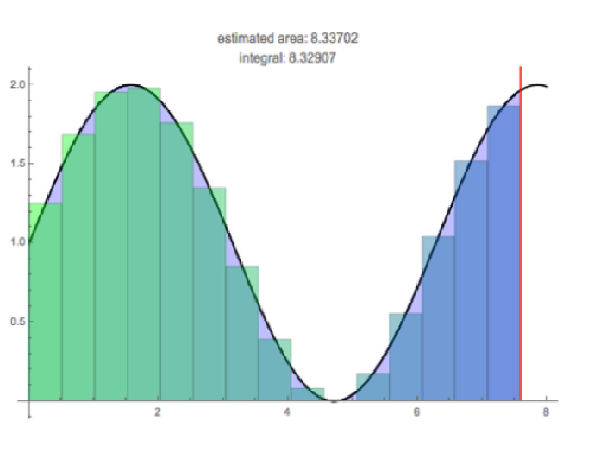
\includegraphics[scale=0.75]{Magazines/img/Vol2/estimate.png}
\end{center}

At the most elementary level, estimation is used in third grade classrooms in the form of rounding. Rounding lets us change numbers to become easier for humans to comprehend and thus manipulate. Even with its simplicity, rounding ubiquitously shows up in daily life: skimming the receipt for validity, say, or deciding about how many books you aim to read in the next year. However, the more interesting usages of estimation are embedded in more complex areas of math. 

Just around this time each year, many Calculus courses around the world will be teaching integration, or the study of finding the area under curves. The classical approach that will be taught is the fundamental theorem of calculus, a neat formula that produces the exact result. Yet, that very theory arose from using estimation. Specifically, after forming small rectangles as shown, the area under the curve will be approximately the total area of the rectangles; this method is called LRAM (“Left Rectangular Approximation Method”, named after Bernhard Riemann , the mathematician who is credited with discovering the method.) When you increase the number of rectangles, the estimation gets more and more precise, approaching the actual area.  

In this way, estimation precedes certainty. How else would you define integral, if not for Riemann sums? But what happens when there is no certainty? In the entire field of statistics, since data is finite and, sometimes, hard to come by,, the statistician’s job is to infer imperfect claims from the available data, rather than calculating absolute truths. As such, no statistics research article in statistics is complete without p-values and confidence rates– there simply isn’t 100 percent confidence. In addition to statistics, some numbers’ exact value cannot be determined, such as $\pi$, and e, to name a few. Moreover, as we’ll see more in depth later, most real-life situations cannot be fully described by tidy equations. Instead, they are better modeled with algorithms that accept and use uncertainty. 

\begin{center}
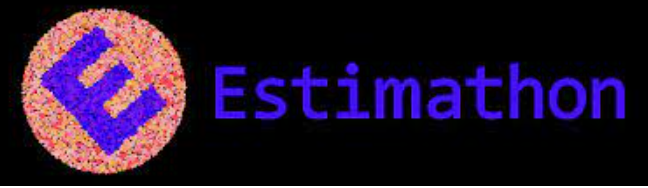
\includegraphics[scale=0.65]{Magazines/img/Vol2/esti2.png}
\end{center}

Even in cases where a clear answer exists, it’s often the case that estimating it is far more time-efficient while still producing a meaningful result. If someone aims to describe the motion of a swinging pendulum (hey, we’re now in physics!), they’ll call on differential equations (equations which involve derivatives of functions). Solving those differential equations would be arduous and annoying, but estimating them is much simpler. This can be done with Taylor series, an extremely powerful estimator tool which can also approximate polynomial functions. To use Taylor series, mathematicians take $f(x)$ on the right hand side of fig. 2, and only use the first few terms–say three. Then, after picking an arbitrary value of a for which the RHS is easily computed, they can then plug in any value for x and get an acutely accurate estimate.

\begin{align*}
    f(x) & =f(a)+\frac{f'(1)}{1!}(x-a)  \\
         & +\frac{f^{(3)}(a)}{3!}(x-a)^3+...
\end{align*} 

Now that we have some sense of a few areas of math where estimation shows up, what is the end result? Can estimation really open new doors? The answer is doubtlessly yes. Even without considering the doors it has already opened, estimation continues to lay the groundwork for mathematicians to sanity-check themselves, and quickens the pace at which they can work. Still, note that that effect is only limited to pure math. To finish, let’s return to applications: ways we use estimation in life.

If you’ve ever toyed with a synthesizer, that’s an estimator function at work, called the Fourier transform. Responses to the COVID-19 pandemic likely were informed by estimations of the potential exponential growth of infection, which at their core are just differential equations. Analysts who estimate the expected growth or fall of a stock power much of the Wall Street economy. Almost every building constructed in the US was guided by an ``Engineer's Estimate,'' wherein engineers predict the total budget needed to complete a project. Moreover, that budget estimate likely used integration (built off simple estimation techniques) to find the shape, and volume, of the building. Love your new TI-84? That calculator deconstructs difficult queries into their corresponding Taylor series, which then approximates the result.

Estimation isn’t just another small tool in a mathematician's kit– it’s more akin to their Phillips-head screwdriver. 


\closearticle
\end{multicols}

\begin{multicols}{2}
\begin{center}
    \noindent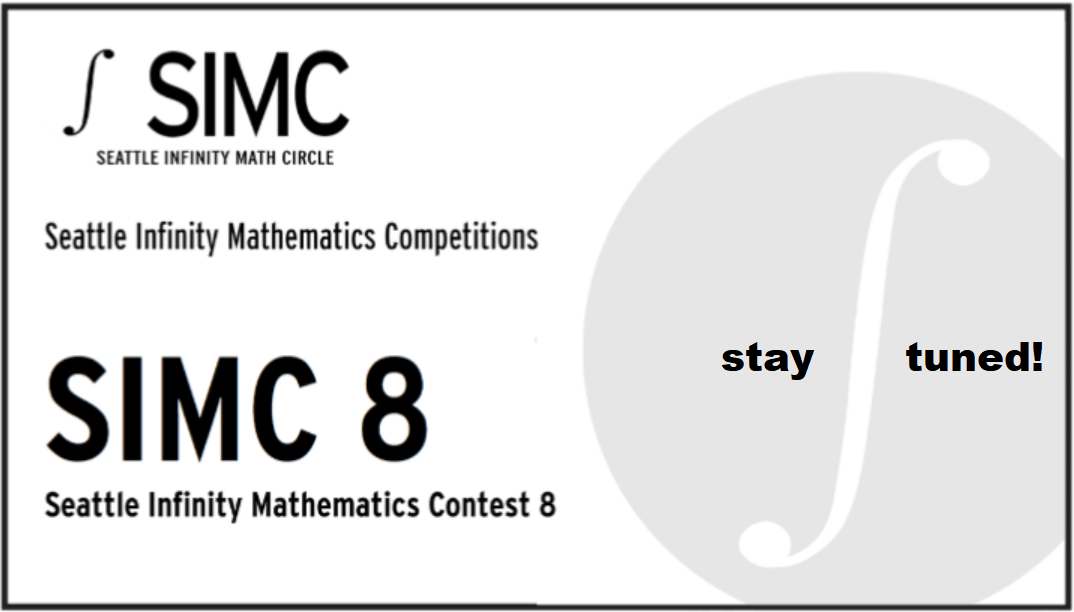
\includegraphics[width=3.0in]{Magazines/img/Vol2/simc8.png}
\end{center}

\begin{center}
    
\includegraphics[width=3.0in]{Magazines/img/Vol2/circle_poster.png}
\end{center}
\clearcolumn
\;
{
\vspace{1.5cm}
%\hspace{24mm} \sc\Large{\textbf{Contact Us}}
\begin{center}
\begin{tabular}{c l}
  
\includegraphics[scale=0.06,valign=c]{Magazines/img/email.png}
    & \href{mailto:seattleinfinitymathcircle@gmail.com}{Email}\\
  \;\\
  
\includegraphics[scale=0.1,valign=c]{Magazines/img/website.png}
    & \href{https://seattleinfinity.org}{Website} \\
  
\includegraphics[scale=0.5,valign=c]{Magazines/img/facebook.png}
    & \href{https://www.facebook.com/simathcircle/}{Facebook} \\
  
\includegraphics[scale=0.5,valign=c]{Magazines/img/insta.png}
    & \href{https://www.instagram.com/seattleinfinitymathcircle/}{Instagram} \\
  
\includegraphics[scale=0.5,valign=c]{Magazines/img/youtube.png}
    & \href{https://www.youtube.com/channel/UCgwA-iysWPc_XG0R0AZ5z5g/videos}{YouTube} \\
  
\includegraphics[scale=0.013,valign=c]{Magazines/img/discord.png}
    & \href{https://discord.gg/2Ma3dURhTt}{Discord} 
\end{tabular}
\end{center} 
}
\end{multicols}
\end{document}
